\section{Durchführung}
\label{sec:Durchführung}

Der Versuch wird gemäß Abbildung \ref{fig:aufbau} aufgebaut. Als Probe wird ein mit Strontium dotierter Kaliumbromid(KBr)-Kristall verwendet.

\begin{figure}
    \centering
    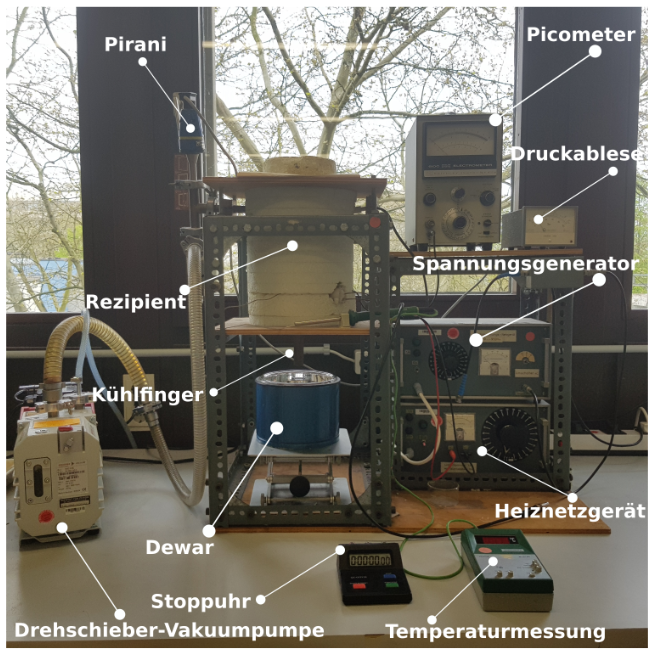
\includegraphics[width=\textwidth]{Bilder/Aufbau.PNG}
    \caption{Aufbau des Versuches.}
    \label{fig:aufbau}
\end{figure}

Die Probe befindet sich innerhalb eines Plattenkondensators auf der unteren Kondensatorplatte. Der Kondensator ist innerhalb eines Rezipienten mit einem Vakuum von etwa $\SI{0.001}{\milli\bar}$, welches von einer angeschlossenen Vakuumpumpe aufrechtgehalten wird. Ohne das Vakuum würde sich auf Grund seiner hygroskopischen Eigenschaftensich auf dem Kristall eine Wasserschicht bilden, welche der Genauigkeit des Versuches schade.
Um die Temperatur des Kristalls zu beeinflussen befinden sich am Boden des Rezipienten eine Heizspule und ein Kühlfinger. Die jeweilige Heizrate kann über den Heizstrom reguliert werden. Zum Kühlen wird der Kühlfinger in flüssigen Stickstoff getaucht. Zum Ablesen der aktuellen Temperatur befindet sich ein Thermoelement auf dem Boden des Rezipienten. 


\begin{figure}
    \centering
    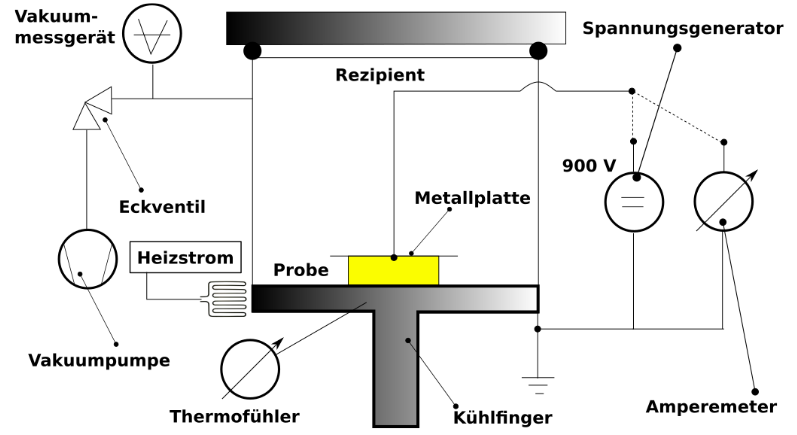
\includegraphics[width=\textwidth]{Bilder/Zeichnung.PNG}
    \caption{Skizzenhafte Darstellung des Aufbaus und Schaltbild der wichtigsten Komponenten.}
    \label{fig:skizze}
\end{figure}

%Was wurde gemessen bzw. welche Größen wurden variiert?